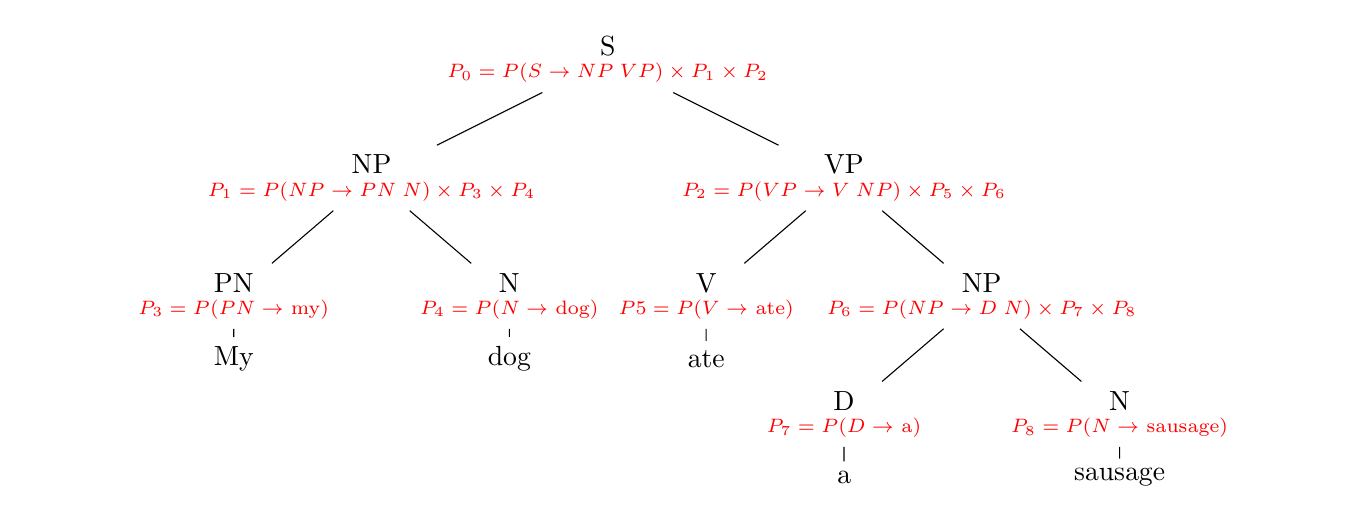
\begin{tikzpicture}
\tikzstyle{level 1}=[sibling distance=60mm]
\tikzstyle{level 2}=[sibling distance=35mm]
\tikzstyle{level 3}=[sibling distance=35mm]
\node {\parbox{5cm}{\centering S\\ \scriptsize\color{red}$P_0 = P(S\rightarrow NP\; VP)\times P_1\times P_2$} }
	child {node (leftnode) {\parbox{5cm}{\centering NP\\ \scriptsize\color{red}$P_1 = P(NP\rightarrow PN \;N)\times P_3\times P_4$}}
		child {node {\parbox{5cm}{\centering PN\\ \scriptsize\color{red}$P_3 =P(PN\rightarrow$ my)}}
			child  [level distance = 8mm] {node {My}}
			}
		child {node {\parbox{5cm}{\centering N\\ \scriptsize\color{red}$P_4 =P(N\rightarrow$ dog)}}
			child[level distance = 8mm] {node {dog}}
			}
		}
	child {node (rightnode) {\parbox{5cm}{\centering VP\\ \scriptsize\color{red}$P_2 = P(VP\rightarrow V\;NP)\times P_5\times P_6$}}
		child {node {\parbox{5cm}{\centering V\\ \scriptsize\color{red}$P5 =P(V\rightarrow$ ate)}}
			child[level distance = 8mm]{node {ate}}
			}
		child {node {\parbox{5cm}{\centering NP\\ \scriptsize\color{red}$P_6 =P(NP\rightarrow D\;N)\times P_7\times P_8$}}
			child {node {\parbox{5cm}{\centering D\\ \scriptsize\color{red}$P_7 =P(D\rightarrow$ a)}}
				child[level distance = 8mm]{node {a}}
				}
			child { node {\parbox{5cm}{\centering N\\ \scriptsize\color{red}$P_8 =P(N\rightarrow$ sausage)}}
				child[level distance = 8mm]{node {sausage}}
				}
			}
		} ;


\end{tikzpicture}
\caption{The probability of a tree is a multiplication of the probability of the production with the probability of its children}